\pagebreak
\markboth{Simulado 2}{}

\num{1} Utilizando um ábaco Miguel representou o seguinte número:

%Pergunta: os alunos conhecem o ábaco? A ilustração é adequada e suficientemente autoexplicativa? Tenho para mim que a resposta a todas essas perguntas é NÃO. 

\begin{figure}[htpb!]
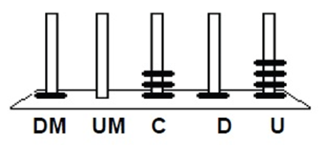
\includegraphics[width=.5\textwidth]{./imgs/mat20.png}
\end{figure}

Qual foi o número que Miguel representou?

\begin{minipage}{.5\textwidth}
\begin{escolha}
\item
  1.314
\item
  4.131
\item
  10.314
\item
  41.301
\end{escolha}
\end{minipage}
\sidetext{SAEB: Compor ou decompor números naturais de até 6 ordens na
forma aditiva, ou em suas ordens, ou em adições e multiplicações.
BNCC: EF05MA01 - Ler, escrever e ordenar números naturais até a ordem das 
centenas de milhar com compreensão das principais características do 
sistema de numeração decimal. 
EF05MA10 - Concluir, por meio de investigações, que a relação de 
igualdade existente entre dois membros permanece ao adicionar, subtrair, 
multiplicar ou dividir cada um desses membros por um mesmo número, para 
construir a noção de equivalência.
EF05MA11 - Resolver e elaborar problemas cuja conversão em sentença 
matemática seja uma igualdade com uma operação em que um dos termos é 
desconhecido.}

\num{2} Isabeli quer colocar o número 380 em uma reta numérica igual à
representada abaixo:

\begin{figure}[htpb!]
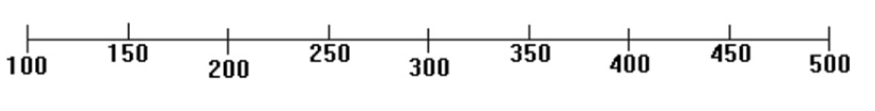
\includegraphics[width=.5\textwidth]{./imgs/mat21.png}
\end{figure}

Entre quais números da reta Isabeli deverá colocar o
número?

\begin{minipage}{.5\textwidth}
\begin{escolha}
\item
  Entre 150 e 200.
\item
  Entre 250 e 300.
\item
  Entre 350 e 400.
\item
  Entre 450 e 500. 
\end{escolha}
\end{minipage}
\sidetext{SAEB: Comparar ou ordenar números racionais (naturais de até
6 ordens, representação fracionária ou decimal finita até a ordem dos
milésimos), com ou sem suporte da reta numérica.
BNCC: EF05MA01 - Ler, escrever e ordenar números naturais até a ordem das 
centenas de milhar com compreensão das principais características do 
sistema de numeração decimal. 
EF05MA10 - Concluir, por meio de investigações, que a relação de 
igualdade existente entre dois membros permanece ao adicionar, subtrair, 
multiplicar ou dividir cada um desses membros por um mesmo número, para 
construir a noção de equivalência.
EF05MA11 - Resolver e elaborar problemas cuja conversão em sentença 
matemática seja uma igualdade com uma operação em que um dos termos é 
desconhecido.}

\num{3} Um lote de 26.104 lápis será embalado em caixas contendo 13
unidades de lápis em cada. Essas caixas serão distribuídas uma para cada
escola estadual que existe na região em que Lucas mora. Quantas escolas
receberão 1 caixa contendo lápis?

\begin{minipage}{.5\textwidth}
\begin{escolha}
\item
  26
\item
  28
\item
  208
\item
  2.008
\end{escolha}
\end{minipage}
\sidetext{SAEB: Resolver problemas de multiplicação ou de divisão,
envolvendo números naturais de até 6 ordens, com os significados de
formação de grupos iguais (incluindo repartição equitativa e medida),
proporcionalidade ou disposição retangular.}



\num{4} Analisando a sequência abaixo pode-se afirmar que o próximo número
será:

(240; 120; 60; 30; ...)

\begin{minipage}{.5\textwidth}
\begin{escolha}
\item
  20
\item
  15
\item
  10
\item
  5
\end{escolha}
\end{minipage}
\sidetext{SAEB: Inferir o padrão ou a regularidade de uma sequência de
números naturais ordenados, objetos ou figuras.}



\num{5} Raquel completará 11 anos daqui 5 semanas e 2 dias. Quantos dias
faltam para ela completar 12 anos?

\begin{minipage}{.5\textwidth}
\begin{escolha}
\item
  37
\item
  27
\item
  17
\item
  7
\end{escolha}
\end{minipage}
\sidetext{SAEB: Determinar o horário de início, o horário de término ou
a duração de um acontecimento.}

\num{6} Um marceneiro quer medir a tábua abaixo, mas esqueceu sua trena.
Dessa forma resolveu usar seu próprio palmo, que mede aproximadamente 
21 cm, como unidade de medida.

\begin{figure}[htpb!]
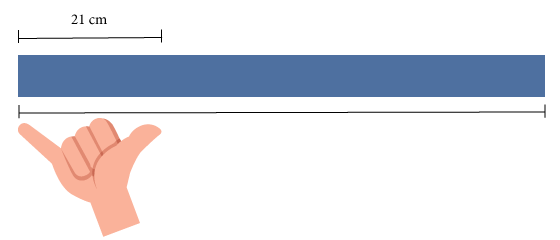
\includegraphics[width=\textwidth]{../ilustracoes/MAT5/SAEB_5ANO_MAT_figura117.png}
\end{figure}

Sabendo-se que ele chegou à conclusão de que a tábua possui o comprimento
de 7 palmos, podemos afirmar que a tábua terá uma medida aproximada
de:

\begin{minipage}{.5\textwidth}
\begin{escolha}
\item
  1,10 m
\item
  1,40 m
\item
  1,50 m
\item
  1,60 m
\end{escolha}
\end{minipage}
\sidetext{SAEB: Estimar/inferir medida de comprimento, capacidade ou
massa de objetos, utilizando unidades de medida convencionais ou não ou
medir comprimento, capacidade ou massa de objetos.
BNCC: EF05MA19 - Resolver e elaborar problemas envolvendo medidas das 
grandezas comprimento, área, massa, tempo, temperatura e capacidade, 
recorrendo a transformações entre as unidades mais usuais em contextos 
socioculturais.}


\num{7} Jonas está marcando, com uma fita, no chão, a letra inicial
do nome de sua mãe.

\begin{figure}[htpb!]
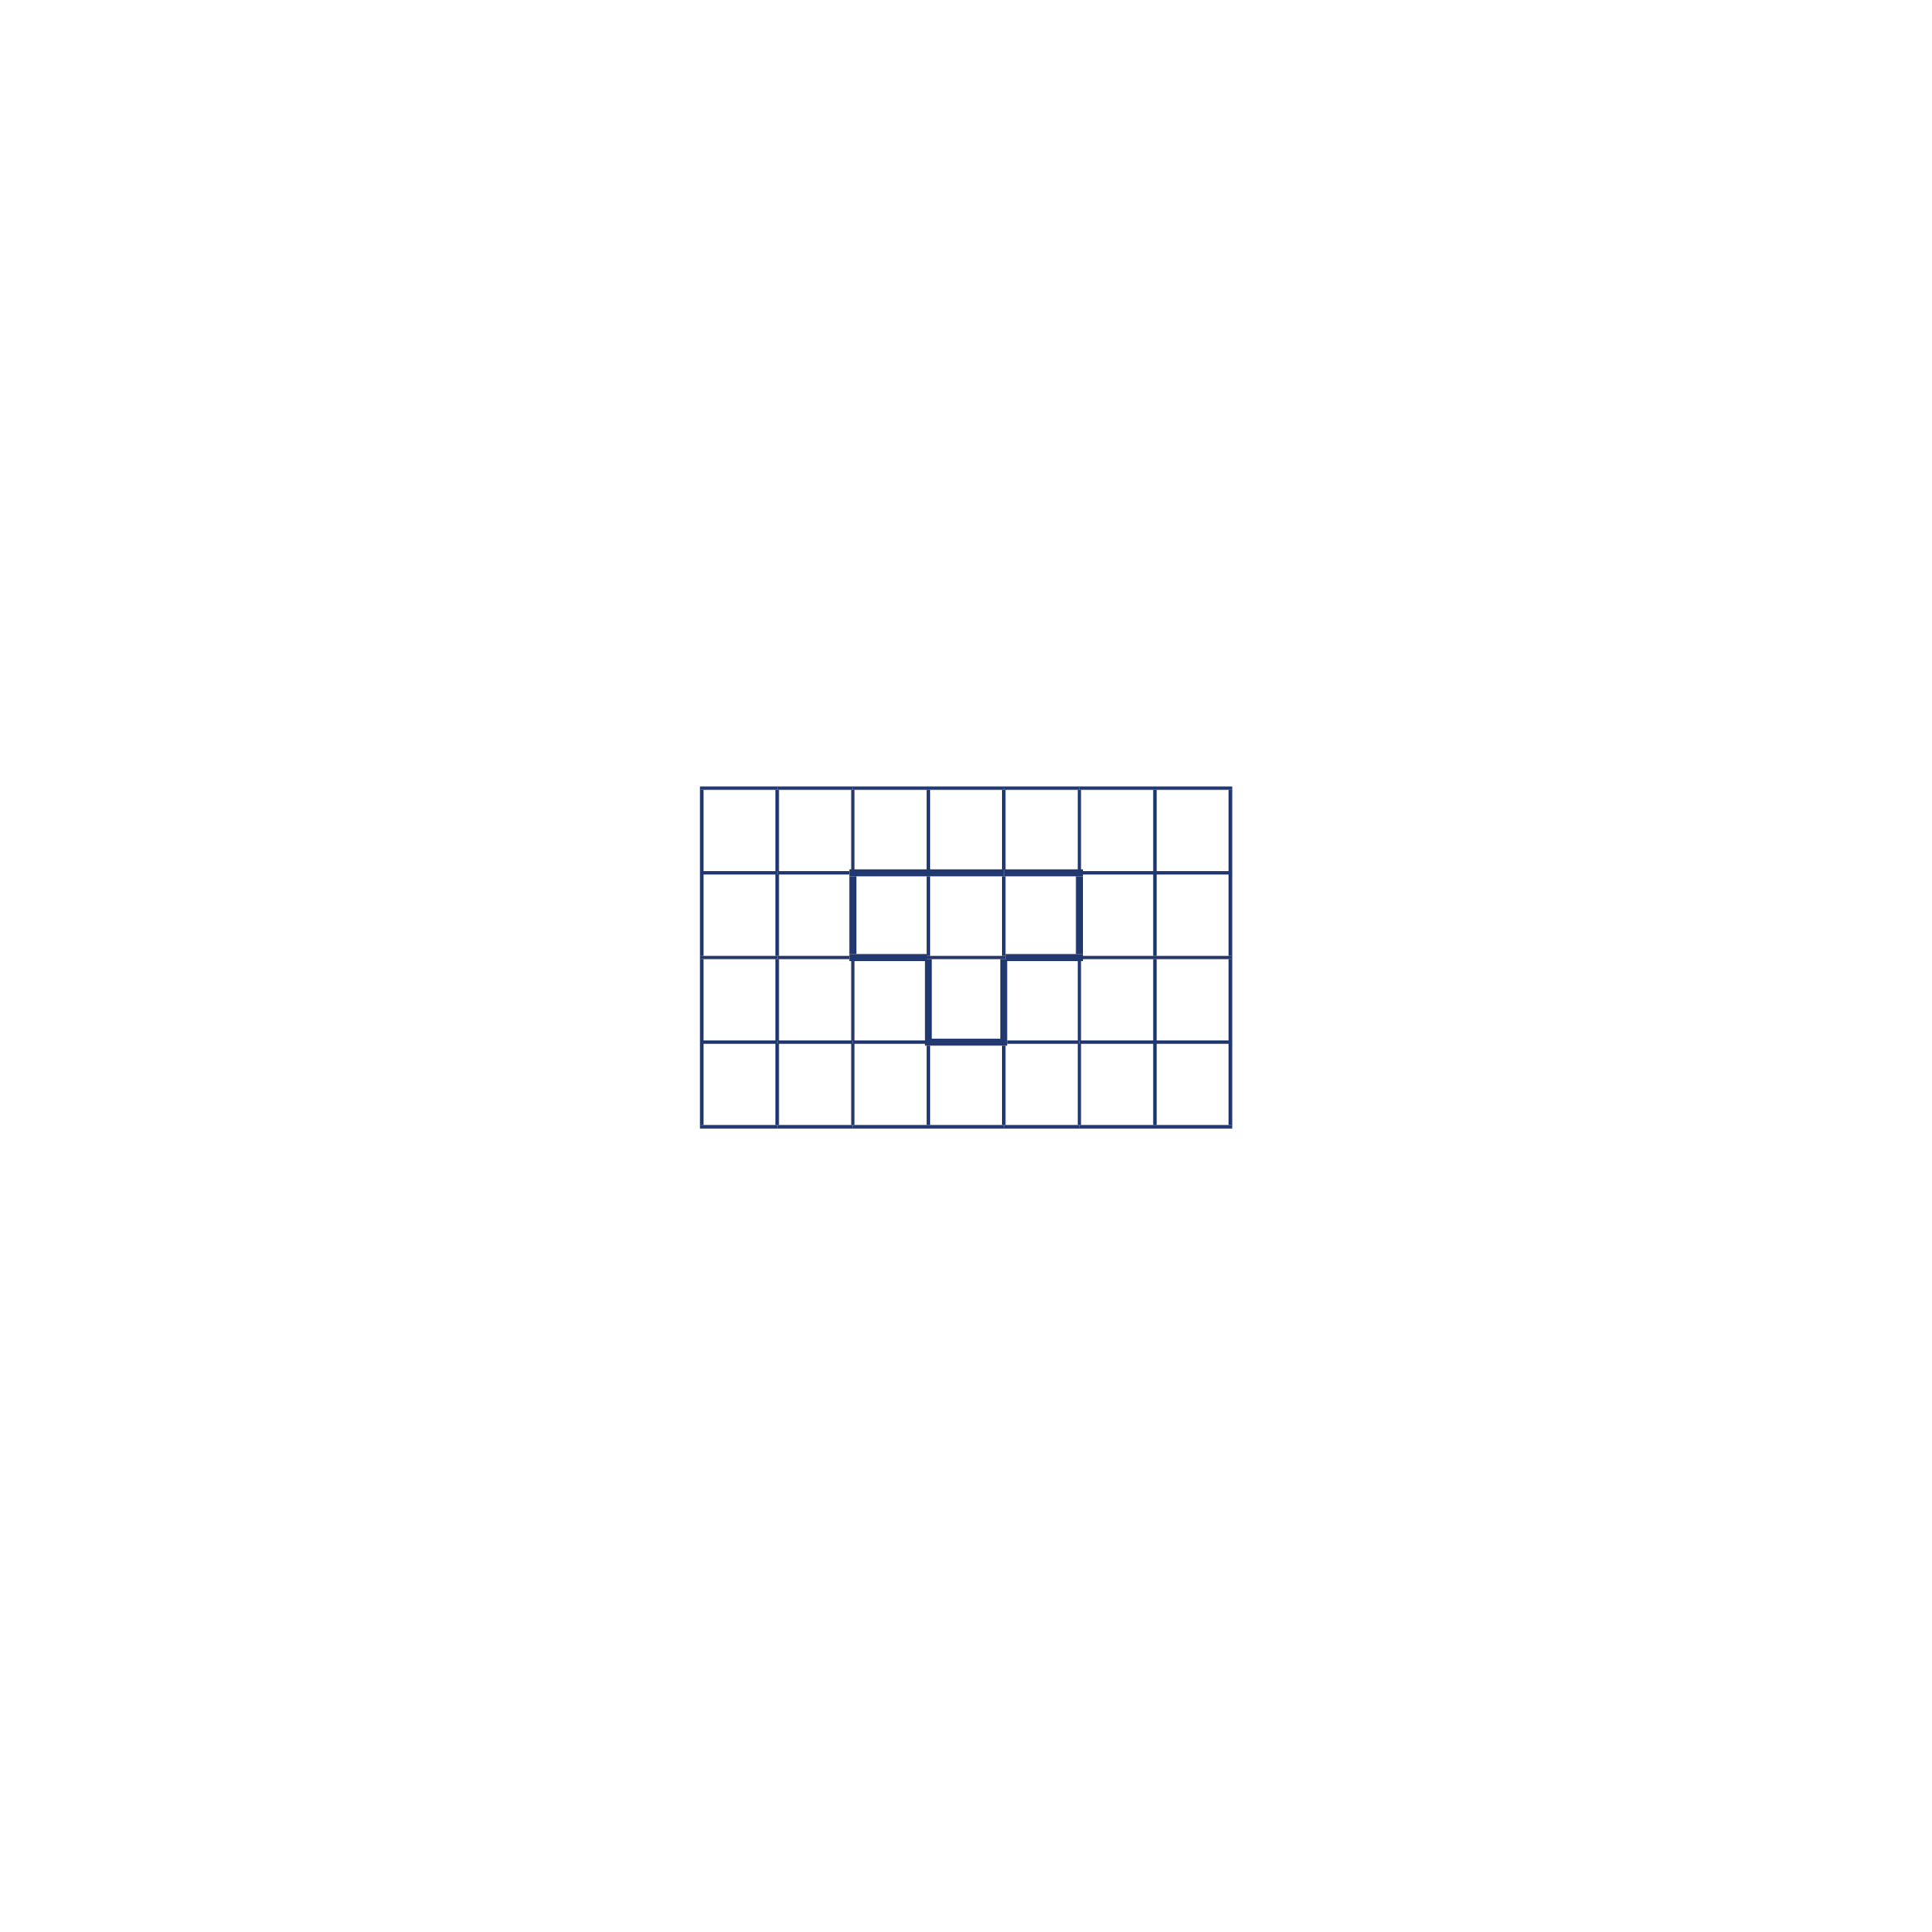
\includegraphics[width=\textwidth]{../ilustracoes/MAT5/SAEB_5ANO_MAT_figura118.png}
\end{figure}

Sabendo-se que cada lado do quadrado que forma o piso mede 1,2 m de
comprimento, quantos metros de fita Jonas precisará para concluir seu
trabalho?

\begin{minipage}{.5\textwidth}
\begin{escolha}
\item
  18
\item
  12
\item
  10
\item
  9
\end{escolha}
\end{minipage}
\sidetext{SAEB: Medir ou comparar perímetro ou área de figuras planas
desenhadas em malha quadriculada.}

\num{8} Vanessa foi à loja de material escolar e comprou os seguintes
itens pelo respectivo preço indicado na figura abaixo:

\begin{figure}[htpb!]
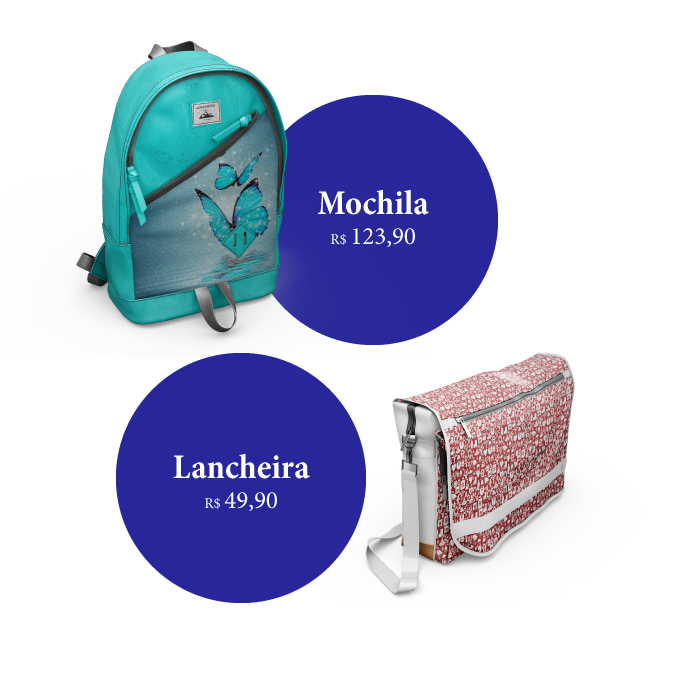
\includegraphics[width=\textwidth]{../ilustracoes/MAT5/SAEB_5ANO_MAT_figura119.png}
\end{figure}
%Abaixo da mochila trocar o preço de 23,90 para 123,90 e o da lancheira trocar de 8,9 para 49,90

Qual foi o valor da compra realizada por Vanessa?

\begin{minipage}{.5\textwidth}
\begin{escolha}
\item
  R\$ 92,80
\item
  R\$ 101,80
\item
  R\$ 132,80
\item
  R\$ 173,80
\end{escolha}
\end{minipage}
\sidetext{SAEB: Resolver problemas que envolvam moedas e/ou cédulas do
sistema monetário brasileiro.}

\num{9} Amanda acaba de jogar um dado, honesto, de 6 faces, em que cada
face contém um número natural distinto de 1 a 6. Qual a probabilidade de,
na face voltada para cima, sair um número menor ou igual a 6?

\begin{minipage}{.5\textwidth}
\begin{escolha}
\item
  0\%
\item
  25\%
\item
  50\%
\item
  100\%
\end{escolha}
\end{minipage}
\sidetext{SAEB: Determinar a probabilidade de ocorrência de um
resultado em eventos aleatórios, quando todos os resultados possíveis
têm a mesma chance de ocorrer (equiprováveis).
BNCC: EF05MA22 - Apresentar todos os possíveis resultados de um
experimento aleatório, estimando se esses resultados são igualmente 
prováveis ou não.
EF05MA23 - Determinar a probabilidade de ocorrência de um resultado em 
eventos aleatórios, quando todos os resultados possíveis têm a mesma 
chance de ocorrer (equiprováveis).}

\num{10} Três alunos realizaram 5 provas cada um e as notas obtidas por
eles se encontram na tabela abaixo:

\begin{tabular}{c|ccccc}
\hline
\multicolumn{1}{l|}{\textbf{Aluno}} & \multicolumn{1}{l}{\textbf{1ª prova}} & \multicolumn{1}{l}{\textbf{2ª prova}} & \multicolumn{1}{l}{\textbf{3ª prova}} & \multicolumn{1}{l}{\textbf{4ª prova}} & \multicolumn{1}{l}{\textbf{5ª prova}} \\ \hline
W & 3 & 4 & 5 & 8 & 7 \\ \hline
X & 5 & 5 & 5 & 10 & 6 \\ \hline
Y & 4 & 9 & 3 & 9 & 5 \\ \hline
Z & 5 & 5 & 8 & 5 & 6 \\ \hline
\end{tabular}

O aluno que será classificado será aquele que tiver a maior
soma de todas as notas, pode-se afirmar que o aluno classificado será o
aluno:

\begin{minipage}{.5\textwidth}
\begin{escolha}
\item
  W
\item
  X
\item
  Y
\item
  Z
\end{escolha}
\end{minipage}
\sidetext{SAEB: Resolver problemas que envolvam dados apresentados
tabelas (simples ou de dupla entrada) ou gráficos estatísticos (barras
simples ou agrupadas, colunas simples ou agrupadas, pictóricos ou de
linhas).
BNCC: EF05MA24 - Interpretar dados estatísticos apresentados em textos, 
tabelas e gráficos (colunas ou linhas), referentes a outras áreas do 
conhecimento ou a outros contextos, como saúde e trânsito, e produzir 
textos com o objetivo de sintetizar conclusões.}

\num{11} Gabriel ganhou de sua avó uma barra de chocolate conforme a 
figura abaixo:

\begin{figure}[htpb!]
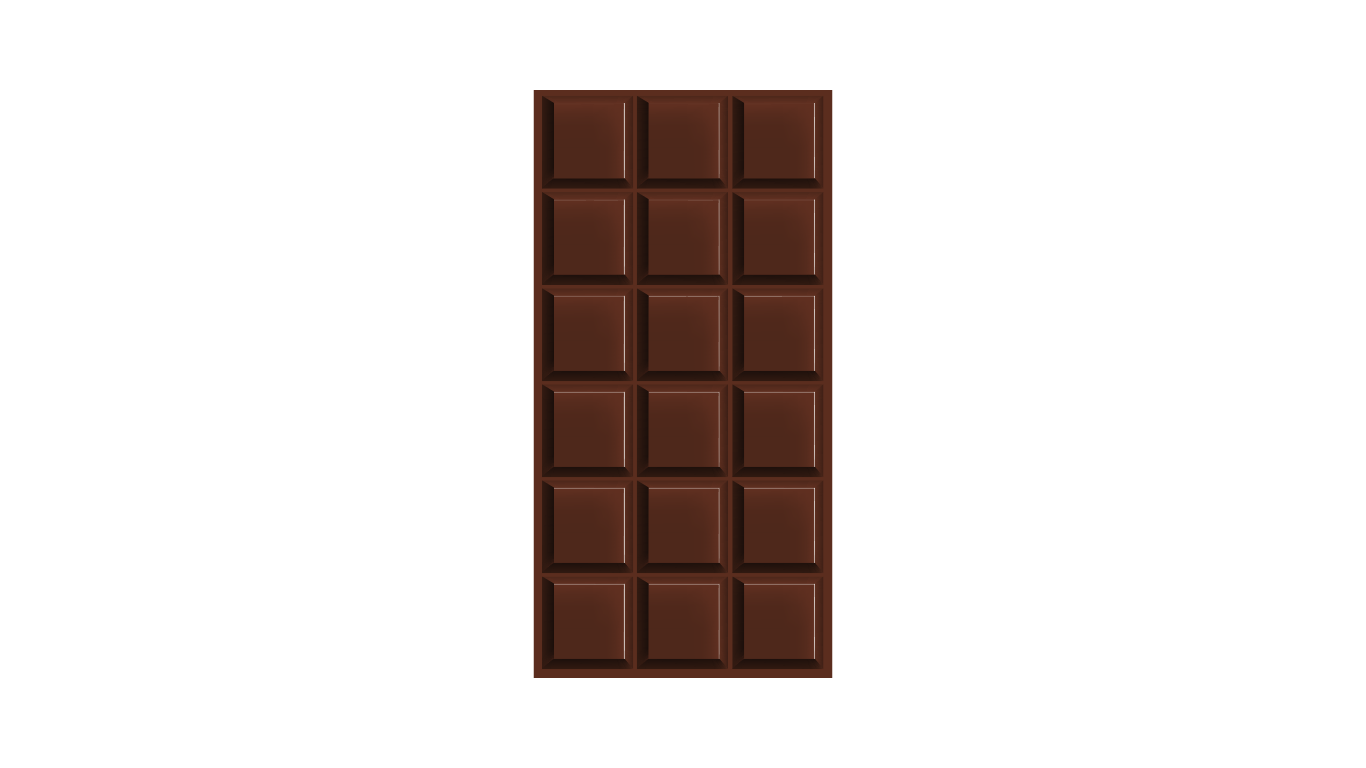
\includegraphics[width=\textwidth]{../ilustracoes/MAT5/SAEB_5ANO_MAT_figura120.png}
\end{figure}

O número de quadradinhos que ele deverá comer para consumir 2/3 do total
da barra de chocolate?

\begin{minipage}{.5\textwidth}
\begin{escolha}
\item
  3
\item
  9
\item
  12
\item
  15
\end{escolha}
\end{minipage}
\sidetext{SAEB: Representar frações menores ou maiores que a unidade
(por meio de representações pictóricas) ou associar frações a
representações pictóricas.
BNCC: EF05MA03 - Identificar e representar frações (menores e maiores que 
a unidade), associando-as ao resultado de uma divisão ou à ideia de parte 
de um todo, utilizando a reta numérica como recurso.
EF05MA04 - Identificar frações equivalentes.
EF05MA06 - Associar as representações 10\%, 25\%, 50\%, 75\% e 100\% 
respectivamente à décima parte, quarta parte, metade, três quartos e um 
inteiro, para calcular porcentagens, utilizando estratégias pessoais, 
cálculo mental e calculadora, em contextos de educação financeira, entre 
outros.}


\num{12} Maria é especialista em fazer um café delicioso. Na receita 
que ela utiliza são utilizadas uma colher de sopa de pó de café para cada
250 ml de água. Se você, utilizando a receita de Maria, pretende
utilizar 750 ml de água, quantas colheres de sopa de pó de café você
deverá utilizar para seguir a receita de Maria?

\begin{minipage}{.5\textwidth}
\begin{escolha}
\item
  2
\item
  3
\item
  4
\item
  5
\end{escolha}
\end{minipage}
\sidetext{SAEB: Resolver problemas que envolvam variação de
proporcionalidade direta entre duas grandezas.
BNCC: EF05MA12 - Resolver problemas que envolvam variação de 
proporcionalidade direta entre duas grandezas, para associar a quantidade 
de um produto ao valor a pagar, alterar as quantidades de ingredientes de 
receitas, ampliar ou reduzir escala em mapas, entre outros.}

\num{13} Para uma competição de xadrez foram inscritos 10 jogadores.
Quantas são as possibilidades de se formar o pódio com o resultado 
final, ou seja, primeiro, segundo e terceiro lugares?
%Acho que a formulação desse enunciado não é clara, mas não consigo redigir melhor. Além disso, sugiro justificativa mais extensa nos gabaritos. Será que a leitura crítica pode resoolver esse problema? (Rogério, 4/3/23, 14h12)

\begin{minipage}{.5\textwidth}
\begin{escolha}
\item
  90
\item
  360
\item
  720
\item
  1 000
\end{escolha}
\end{minipage}
\sidetext{SAEB: Resolver problemas simples de contagem (combinatória).
BNCC: EF05MA09 - Resolver e elaborar problemas simples de contagem 
envolvendo o princípio multiplicativo, como a determinação do número de 
agrupamentos possíveis ao se combinar cada elemento de uma coleção com 
todos os elementos de outra coleção, por meio de diagramas de árvore ou 
por tabelas.}

\num{14} Pela manhã, Ricardo abasteceu seu carro, pois o tanque estava
totalmente vazio. Ele gastou R\$ 191,88 para encher o tanque
completamente.

Sabendo-se que o preço do litro do combustível utilizado por Ricardo
custa R\$ 3,69, quantos litros de combustível couberam no carro de
Ricardo?

\begin{minipage}{.5\textwidth}
\begin{escolha}
\item
  25
\item
  34
\item
  46
\item
  52
\end{escolha}
\end{minipage}
\sidetext{SAEB: Resolver problemas de multiplicação ou de divisão,
envolvendo números racionais apenas na representação decimal finita até
a ordem dos milésimos, com os significados de formação de grupos iguais
(incluindo repartição equitativa de medida), proporcionalidade ou
disposição retangular.
BNCC: EF05MA07 - Resolver e elaborar problemas de adição e subtração com 
números naturais e com números racionais, cuja representação decimal seja 
finita, utilizando estratégias diversas, como cálculo por estimativa, 
cálculo mental e algoritmos.
EF05MA08 - Resolver e elaborar problemas de multiplicação e divisão com 
números naturais e com números racionais cuja representação decimal é 
finita (com multiplicador natural e divisor natural e diferente de zero), 
utilizando estratégias diversas, como cálculo por estimativa, cálculo 
mental e algoritmos.}


\num{15} Leia um trecho de artigo científico.
\begin{quote}
  {[}\ldots{}{]} no desenvolvimento da dança são encontrados vários
  descaminhos, entre eles estão os fatores que apontam para a exclusão
  da dança nos planejamentos de educação física {[}\ldots{}{]}

{[}\ldots{}{]} perguntamos se acham que exista algum preconceito dos alunos a
respeito do conteúdo dança e {[}\ldots{}{]} pedimos para dizer quais os
preconceitos encontrados, e 100\% deles responderam que o maior
preconceito está ligado ao gênero por parte dos meninos.

\fonte{Vinicius Giacomini de Castro, Diogo Santos Silva e Marli das Graças Júlio. EFDEPORTES. O preconceito da dança nas escolas.
Revista Digital. Buenos Aires, Año 15, Nº 150, Noviembre de 2010.
Disponível em: \emph{
https://www.efdeportes.com/efd150/o-preconceito-da-danca-nas-escolas.htm}.
Acesso em: 14 fev. 2023.}
\end{quote}

\noindent{}Com base no texto, o pensamento estereotipado na dança é achar que é um(a)

\begin{escolha}
\item modalidade desconhecida por parte dos alunos.

\item esporte evitado na escola.

\item atividade de que os homens não podem participar.

\item prática corporal voltada para mulheres.
\end{escolha}

\coment{SAEB: Avaliar situações de preconceito no contexto das práticas
corporais.

BNCC: EF35EF09 -- Experimentar, recriar e fruir danças populares do
Brasil e do mundo e danças de matriz indígena e africana, valorizando e
respeitando os diferentes sentidos e significados dessas danças em suas
culturas de origem.}

\num{16} Leia o texto.
\begin{quote}
  Acontece na próxima sexta-feira, {[}\ldots{}{]} no Ginásio Municipal de
  Esportes Domingos Angelino Régis, no Centro de Navegantes, um evento
  direcionado aos alunos das 8ª Séries da Rede Municipal de Ensino, que
  tem por objetivo despertar nos estudantes a importância do esporte
  como mecanismo de motivação, superação e combate ao preconceito. O
  evento também vai contar com a participação de atletas do paradesporto
  e da Apae de Navegantes.

{[}\ldots{}{]} no local haverá uma apresentação das equipes de Basquete e
Handebol do Clube Roda Solta {[}\ldots{}{]}.

\fonte{Prefeitura de Navegantes. Alunos participam de evento sobre motivação e superação através do esporte. Disponível em: \emph{
https://www.navegantes.sc.gov.br/noticia/9274/alunos-participam-de-evento-sobre-motivacao-e-superacao-atraves-do-esporte}.
Acesso em: 15 fev. 2023.}
\end{quote}

\noindent{}O evento citado, para os alunos, serviu para que eles

\begin{escolha}
\item praticassem novos esportes.

\item promovessem a conscientização dos paratletas.

\item entendessem os benefícios dos esportes.

\item ajudassem na organização do evento.
\end{escolha}

\coment{SAEB: Avaliar meios para superar situações de preconceito no contexto
das práticas corporais.

BNCC: EF35EF06 -- Diferenciar os conceitos de jogo e esporte,
identificando as características que os constituem na contemporaneidade
e suas manifestações (profissional e comunitária/lazer).}

\num{17} Leia sobre as cantigas de roda.
\begin{quote}
  {[}\ldots{}{]} caso das cantigas de roda que, historicamente fazem parte
  das tradicionais brincadeiras infantis {[}\ldots{}{]}

{[}\ldots{}{]} Ficou claro que a cantiga de roda é inserida em sala de aula
para promover o lúdico para a criança. {[}\ldots{}{]} Nem todas as crianças
sabem cantar muitas músicas que são tidas como tradicionais. Isso porque
o envolvimento das mesmas com tecnologias pode as estar afastando de
tradições ricas e importantes como são as cantigas de roda. {[}\ldots{}{]}

\fonte{UFG. Patrimônio, direitos culturais e cidadania. As cantigas de roda como manifestações do patrimônio cultural: o papel
da escola na perpetuação dessa cultura. Disponível em: \emph{
https://publica.ciar.ufg.br/ebooks/eipdcc-propostas-pratica-acoesdialogicas/artigos/artigo34.html}.
Acesso em: 15 fev. 2023.}
\end{quote}

\noindent{}Com base no texto, podemos perceber que a brincadeira tradicional citada

\begin{escolha}
\item está sendo esquecida por parte dos alunos.

\item vem ganhando popularidade por causa da tecnologia.

\item apresenta algumas desvantagens para os estudantes.

\item aparece como uma atividade pouco usada na escola.
\end{escolha}

\coment{SAEB: Identificar as brincadeiras e os jogos populares como patrimônio
histórico-cultural.

BNCC: EF35EF01 -- Experimentar e fruir brincadeiras e jogos populares do
Brasil e do mundo, incluindo aqueles de matriz indígena e africana, e
recriá-los, valorizando a importância desse patrimônio histórico
cultural.}


\num{18} O coração, sangue e vasos sanguíneos compõem a estrutura do
sistema circulatório. Em conjunção com outros sistemas do organismo, o
sistema circulatório participa da nutrição das células do corpo humano,
transportando nutrientes para músculos e órgãos.

Esse sistema também tem por função a

\begin{minipage}{.5\textwidth}
\begin{escolha}
\item produção de gases.

\item eliminação de toxinas.

\item maturação de nutrientes.

\item digestão de alimentos.
\end{escolha}
\end{minipage}
\sidetext{BNCC: EF05CI06 - Selecionar argumentos que justifiquem por
que os sistemas digestório e respiratório são considerados
corresponsáveis pelo processo de nutrição do organismo, com base na
identificação das funções desses sistemas.}

\num{19} Um relatório de especialistas descreveu que, às margens de
um rio brasileiro, há pouca concentração vegetal, e uma extensa
deterioração do solo, tornando-o improdutivo. Além disso, o acúmulo de
lixo na região é muito grande. Eles concluíram que a área foi afetada
pela atividade humana e entregaram uma série de medidas para as
autoridades, visando evitar maiores problemas.

\begin{longtable}[]{@{}ll@{}}
\toprule
\textbf{Medida} & \textbf{Justificativa}\tabularnewline
Cultivo de plantas leguminosas. & Adubar o solo
empobrecido.\tabularnewline
Instalação de barreiras de contenção. & Impedir o acúmulo de detritos no
rio.\tabularnewline
Remoção do lixo acumulado na região. & Prevenir o transporte do lixo até
o rio.\tabularnewline
Plantio de árvores no solo recuperado. & Reflorestar o entorno do
rio.\tabularnewline
\bottomrule
\end{longtable}

Tais medidas buscam prevenir o processo de

\begin{minipage}{.5\textwidth}
\begin{escolha}
\item ressecamento de nascentes.

\item cruzamento de correntes oceânicas.

\item escoamento das águas.

\item assoreamento do rio.
\end{escolha}
\end{minipage}
\sidetext{BNCC: EF05CI03 - Selecionar argumentos que justifiquem a
importância da cobertura vegetal para a manutenção do ciclo da água, a
conservação dos solos, dos cursos de água e da qualidade do ar
atmosférico.}

\num{20} Em 21/12/2022, o Brasil teve o dia mais longo e a noite
mais curta do ano. Esse período marcou a passagem da primavera para o
verão no país, graças à maior incidência de luz do sol no Hemisfério Sul
e à inclinação do planeta Terra. Esse fenômeno é conhecido como
solstício de verão.

No Hemisfério Norte, qual estação do ano se iniciou no mesmo dia?

\begin{minipage}{.5\textwidth}
\begin{escolha}
\item Primavera.

\item Outono.

\item Verão.

\item Inverno.
\end{escolha}
\end{minipage}
\sidetext{BNCC: EF05CI11 - Associar o movimento diário do Sol e das
demais estrelas no céu ao movimento de rotação da Terra.}